\documentclass[11pt]{article}

\usepackage[margin=1in]{geometry}
\usepackage{booktabs}
\usepackage{hyperref}
\usepackage{caption}
\usepackage{graphicx}
\usepackage{microtype}

\title{\bfseries Supplementary Information\\Background matching audits mass spectral antimicrobial resistance prediction}
\author{}
\date{}

\begin{document}
\maketitle

\section*{Supplementary Note 1: Why background matching is needed}

Raw external AUC answers whether a model ranks resistant isolates above susceptible isolates at a target site. It does not answer whether that ranking is driven by focal-drug biology or by the resistant population in which the label occurs. In bacterial clinical data, resistance labels are structured by lineage, mobile elements, local prescribing ecology and co-resistance. A MALDI-TOF model can exploit this structure because spectra encode abundant cellular proteins and lineage-associated peak patterns.

The background-matched audit controls the observable co-resistance component of this structure. For each focal drug, isolates are grouped by the AST labels of the other drugs in the same panel. The focal drug is excluded from the signature. Within valid strata, resistant and susceptible isolates have the same observed co-resistance background. If the model still separates them, it has residual within-background signal. If performance collapses, the original raw AUC was likely driven partly by background differences between strata.

\section*{Supplementary Note 2: Interpretation of the three AUCs}

\textbf{Raw AUC} is computed over all available isolates for the focal organism-drug-site comparison. It is the standard external performance metric.

\textbf{Matched AUC} is computed after removing strata that lack enough resistant and susceptible isolates for the focal drug. It asks whether performance remains in the subset where within-background comparisons are possible.

\textbf{Background-centered AUC} subtracts the mean model score within each valid background stratum before pooling and recomputing AUC. It is the strictest metric because it removes score shifts shared by all isolates in a background stratum.

\section*{Supplementary Note 3: How to read low-retention rows}

Low retention is not a model failure. It is an audit limitation. If a drug-site pair has few strata containing both resistant and susceptible isolates, then the data do not support a strong within-background conclusion. These rows should be reported as cautionary rather than interpreted as biological evidence.

This is why DRIAMS-B ciprofloxacin is not used as main evidence despite a high centered AUC. The estimate is based on only 25 matched isolates and one valid stratum. The method intentionally makes this visible.

\section*{Supplementary Figure S1: Cross-resistance network}

\begin{figure}[ht]
\centering
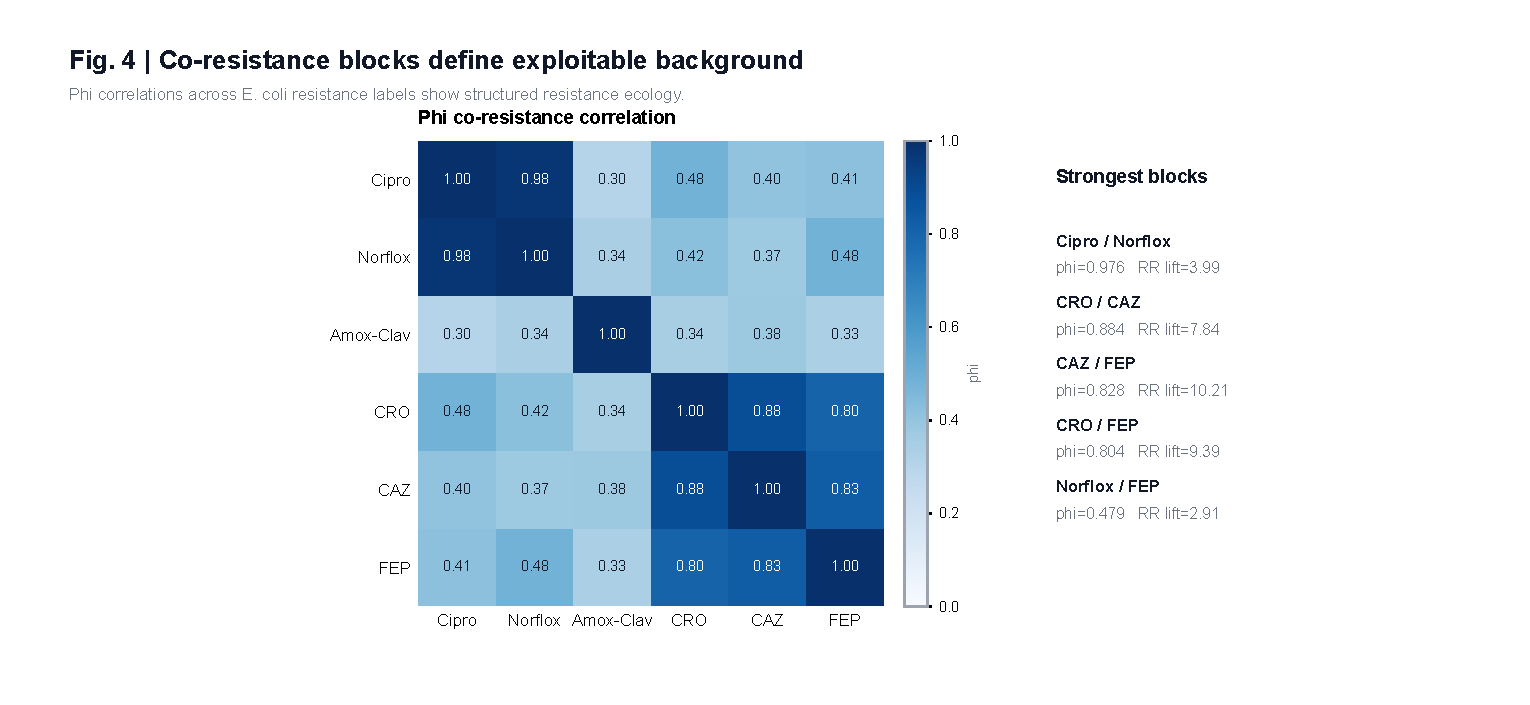
\includegraphics[width=\linewidth]{../figures/figure_4_cross_resistance_network.pdf}
\caption{\textbf{Cross-resistance network in the expanded \textit{E.~coli} panel.} Edge width and shading encode pairwise phi correlation. Two strong blocks are evident: a fluoroquinolone block (ciprofloxacin/norfloxacin, $\phi = 0.976$) and an extended-spectrum cephalosporin block (ceftriaxone, ceftazidime and cefepime, $\phi = 0.804$--$0.884$). These co-resistance structures provide exploitable background signal for any model predicting drugs within either block. Source data: \texttt{source\_data\_fig4\_cross\_resistance\_edges\_all\_sites.csv}.}
\label{suppfig:cross-resistance}
\end{figure}

\section*{Supplementary Figure S2: Falsification controls}

\begin{figure}[ht]
\centering
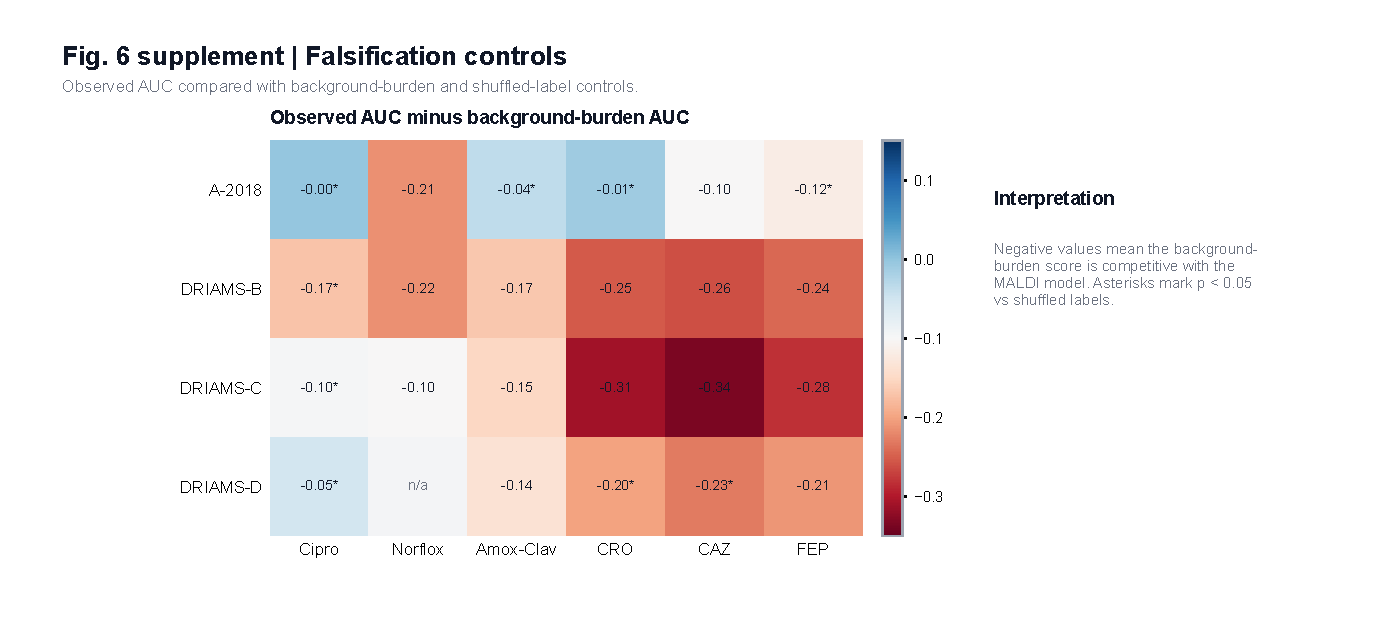
\includegraphics[width=\linewidth]{../figures/figure_6_falsification_controls.pdf}
\caption{\textbf{Falsification controls for background-burden and within-background shuffled-label signal.} Negative observed-minus-burden values indicate rows where a simple non-focal resistance-burden score is competitive with the MALDI model. Shuffled-label controls preserve background strata while disrupting focal-label association.}
\label{suppfig:falsification-controls}
\end{figure}

\section*{Supplementary Figure S3: \textit{S. aureus}/oxacillin audit}

\begin{figure}[ht]
\centering
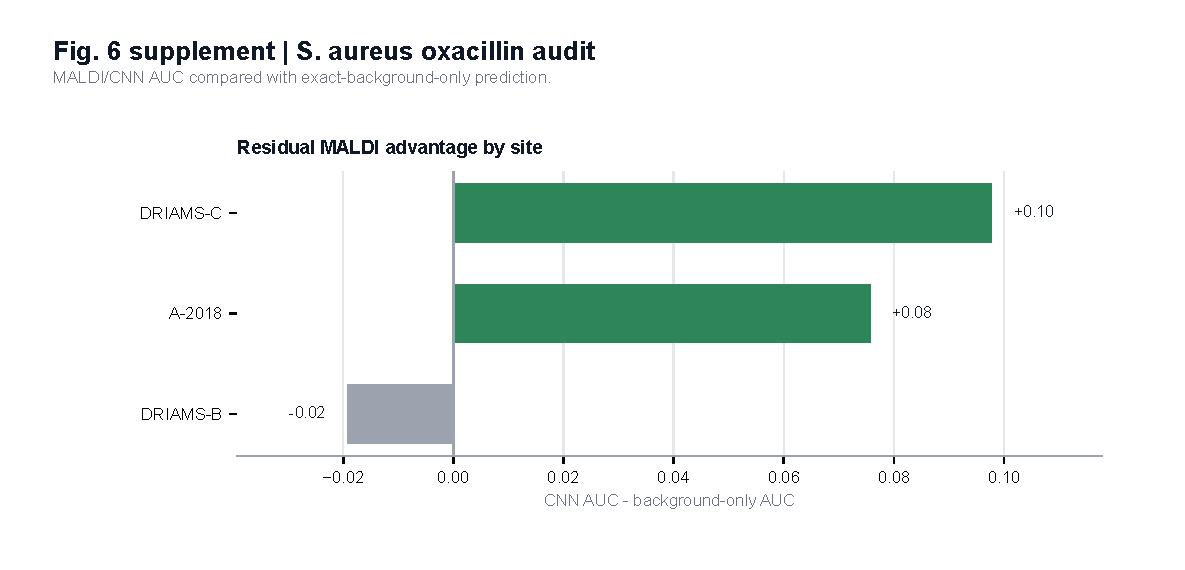
\includegraphics[width=\linewidth]{../figures/figure_6_saureus_oxacillin_audit.pdf}
\caption{\textbf{\textit{S. aureus}/oxacillin second-organism audit.} Oxacillin predictions retained background-centered signal at A-2018 and DRIAMS-C and exceeded the exact-background no-spectrum baseline at both sites. DRIAMS-B is shown for completeness but has only one valid matched stratum. This analysis demonstrates that the audit applies beyond \textit{E. coli}; it is not a systematic multi-organism atlas.}
\label{suppfig:saureus-oxa}
\end{figure}

\section*{Supplementary Figure S4: Three-way decomposition}

\begin{figure}[ht]
\centering
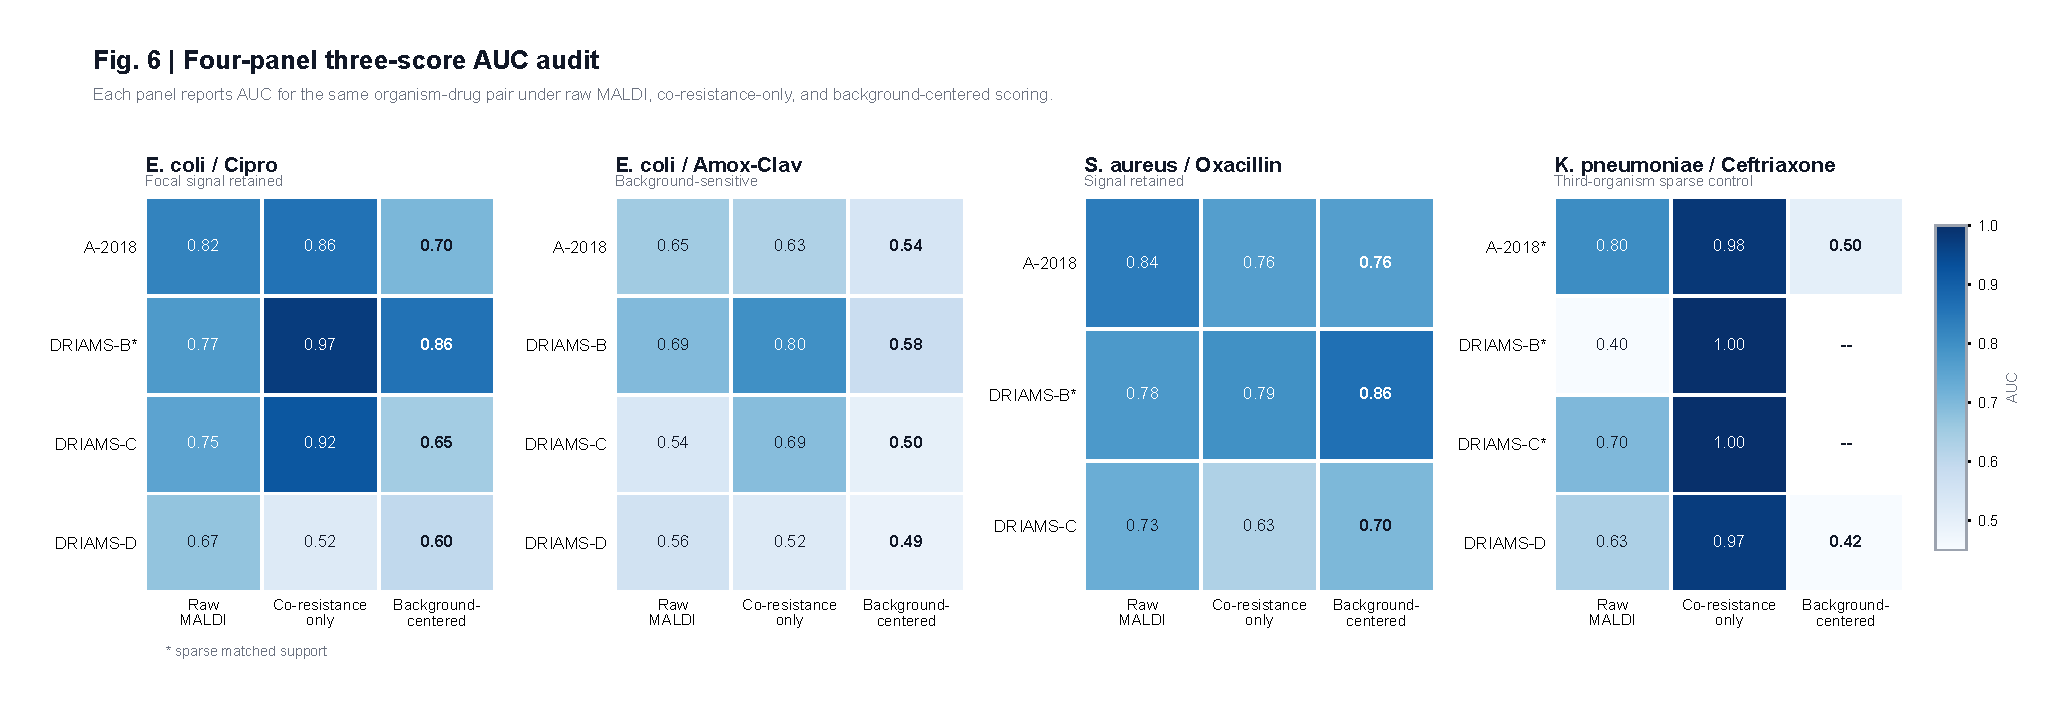
\includegraphics[width=\linewidth]{../figures/figure_6_three_way_decomposition.pdf}
\caption{\textbf{Four-panel three-score decomposition of MALDI and AST-background signal.} Each panel reports raw MALDI AUC, no-spectrum co-resistance-only AUC and background-centered MALDI AUC for the same organism-drug-site rows. The current version includes the \textit{K. pneumoniae}/ceftriaxone panel as a third-organism sparse-control case.}
\label{suppfig:three-way}
\end{figure}

\section*{Supplementary Figure S5: Deployment decision flow}

\begin{figure}[ht]
\centering
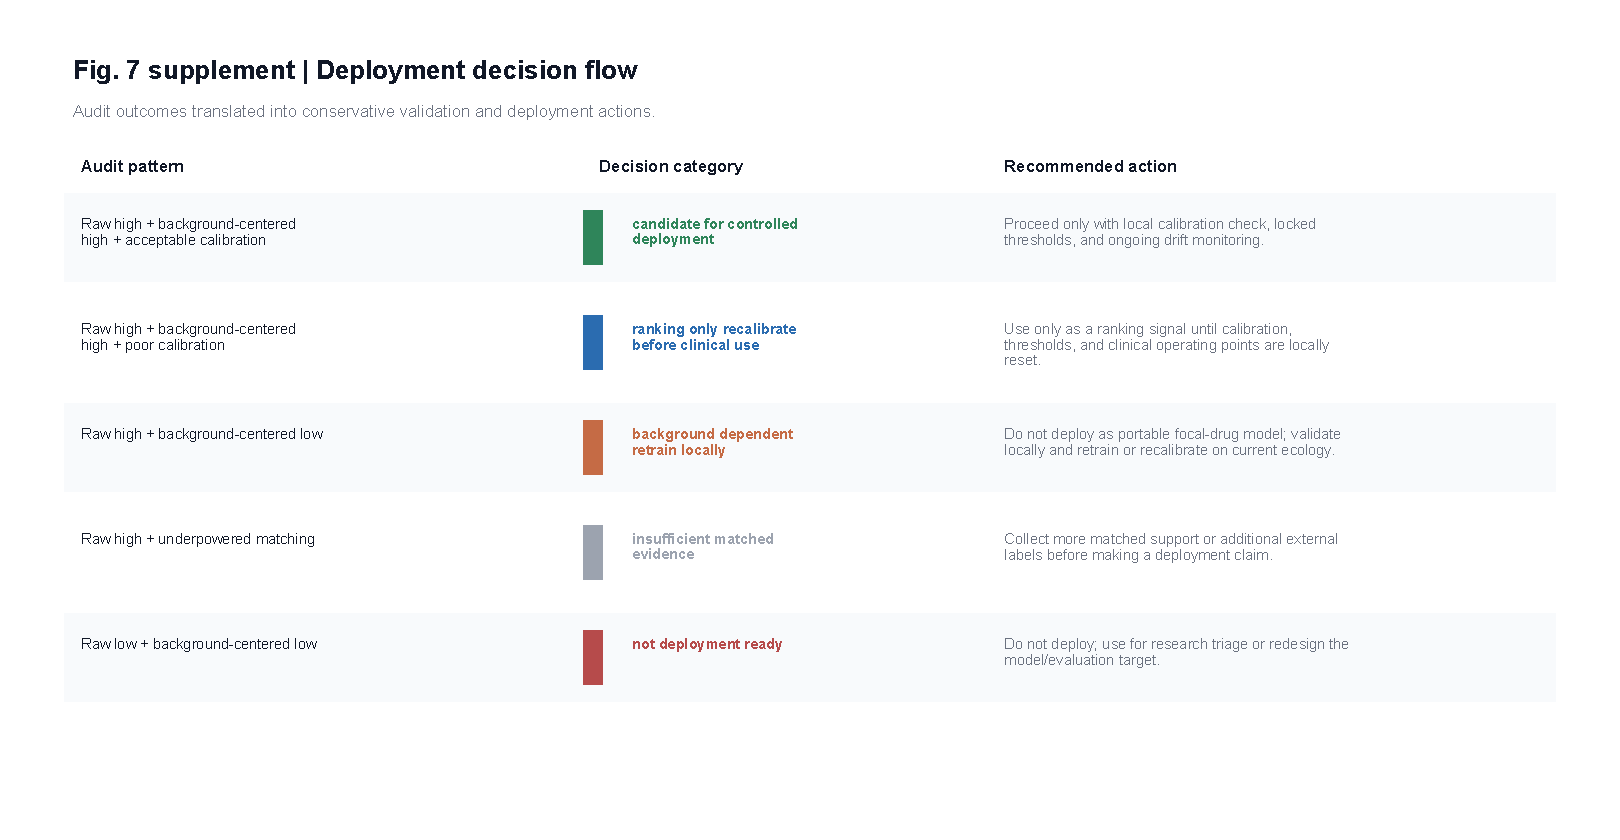
\includegraphics[width=\linewidth]{../figures/figure_7_deployment_decision_flow.pdf}
\caption{\textbf{Deployment decision flow.} Audit outcomes map to conservative validation, recalibration, retraining or no-deployment actions depending on retained signal, calibration and matched-support adequacy.}
\label{suppfig:deployment-flow}
\end{figure}

\section*{Supplementary Figure S6: Framework comparison}

\begin{figure}[ht]
\centering
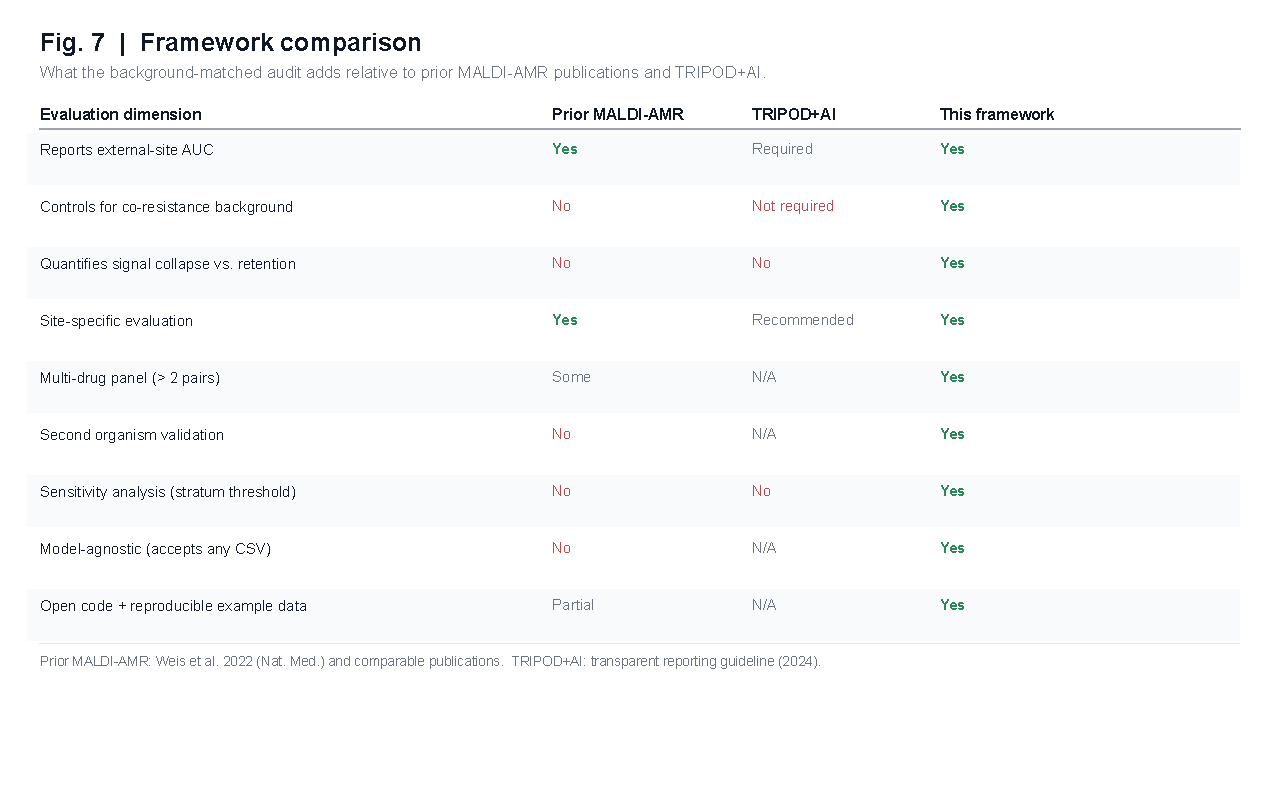
\includegraphics[width=\linewidth]{../figures/figure_7_framework_comparison.pdf}
\caption{\textbf{Framework comparison.} The background-matched audit is positioned relative to prior MALDI-AMR evaluation and general clinical prediction reporting frameworks.}
\label{suppfig:framework-comparison}
\end{figure}

\section*{Supplementary Figure S7: Audit atlas summary}

\begin{figure}[ht]
\centering
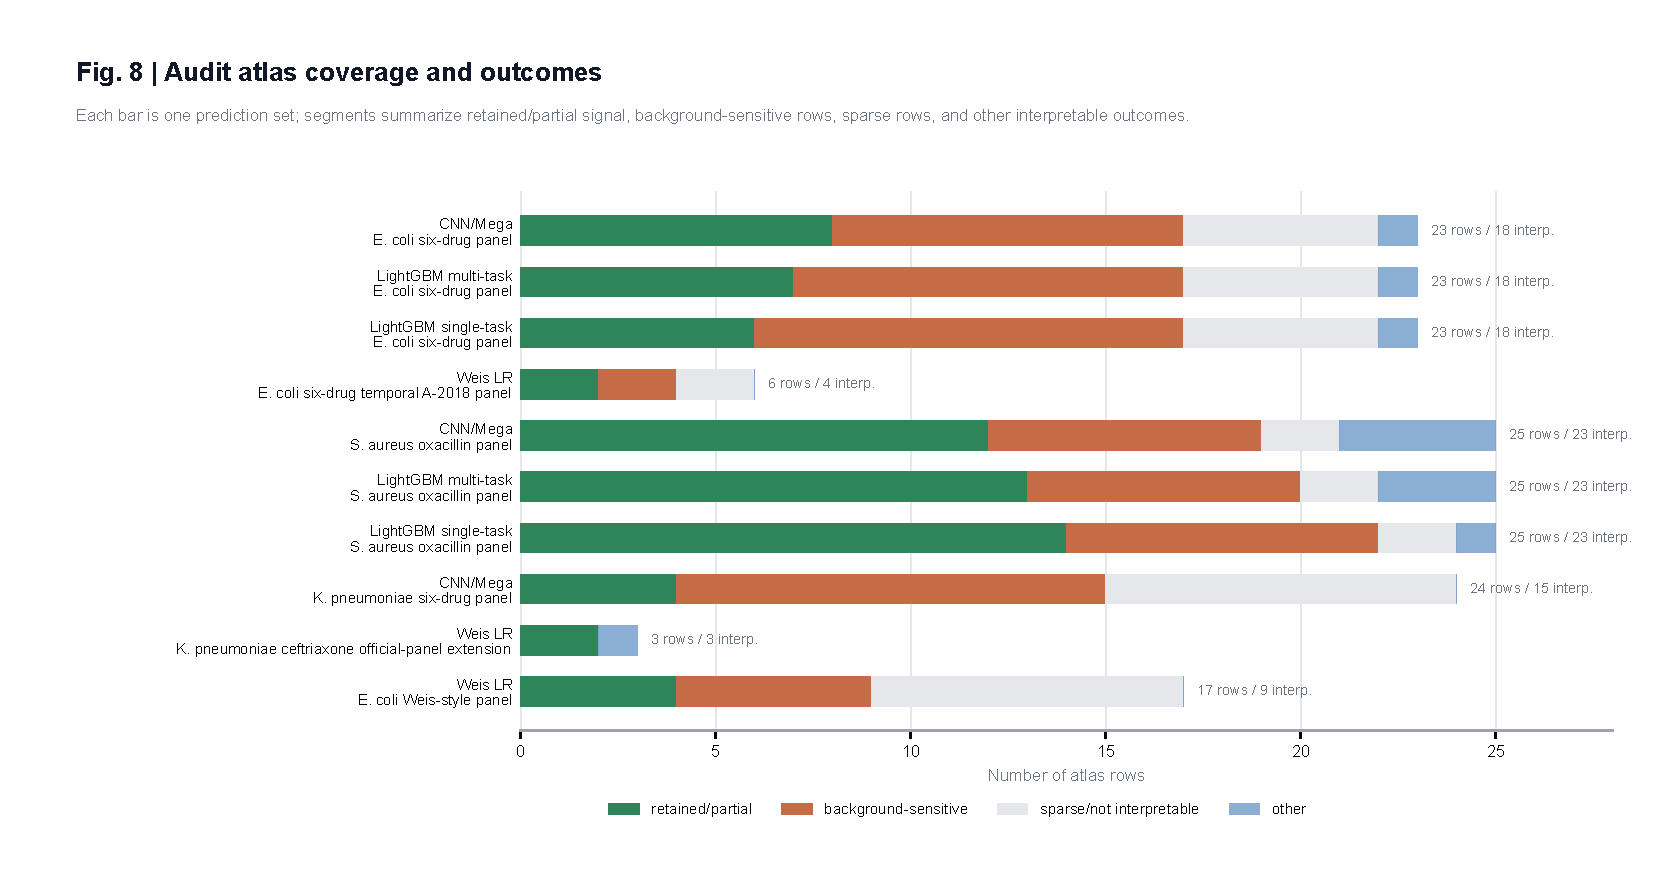
\includegraphics[width=\linewidth]{../figures/figure_8_audit_atlas_summary.pdf}
\caption{\textbf{Audit atlas coverage and outcomes.} Each bar summarizes one prediction set in the current atlas. Segments show retained or partial residual signal, background-sensitive rows, sparse or non-interpretable rows and other interpretable outcomes.}
\label{suppfig:audit-atlas}
\end{figure}

\section*{Supplementary Table 1: Claim guardrails}

\input{../tables/table_6_claim_guardrails.tex}

\section*{Supplementary Table 2: Compact model-family table}

\input{../tables/table_2_model_replication_compact.tex}

\section*{Supplementary Table 3: Full \textit{K. pneumoniae} six-drug audit}

\begin{table}[ht]
\centering
\scriptsize
\caption{Full K. pneumoniae six-drug audit results and Weis ceftriaxone extension.}
\label{tab:klebsiella-panel-audit}
\resizebox{\linewidth}{!}{%
\begin{tabular}{lllrrrrll}
\toprule
Model & Site & Drug & Raw AUC & Centered AUC & Background AUC & Retention (\%) & Strata & Interpretation \\
\midrule
CNN/Mega & A-2018 & Amox-Clav & 0.743 & 0.532 & 0.885 & 79.6 & 3 & background only competitive and weak residual \\
CNN/Mega & DRIAMS-B & Amox-Clav & 0.331 & -- & 0.994 & 0.0 & 0 & not interpretable or sparse \\
CNN/Mega & DRIAMS-C & Amox-Clav & 0.646 & 0.473 & 0.931 & 38.6 & 3 & background only competitive and weak residual \\
CNN/Mega & DRIAMS-D & Amox-Clav & 0.612 & 0.484 & 0.888 & 93.2 & 6 & background only competitive and weak residual \\
CNN/Mega & A-2018 & FEP & 0.896 & -- & 0.999 & 0.0 & 0 & not interpretable or sparse \\
CNN/Mega & DRIAMS-B & FEP & 0.443 & -- & 1.000 & 0.0 & 0 & not interpretable or sparse \\
CNN/Mega & DRIAMS-C & FEP & 0.649 & -- & 1.000 & 0.0 & 0 & not interpretable or sparse \\
CNN/Mega & DRIAMS-D & FEP & 0.647 & 0.396 & 0.998 & 0.9 & 1 & background only competitive and weak residual \\
CNN/Mega & A-2018 & CAZ & 0.809 & 0.208 & 0.996 & 2.1 & 1 & background only competitive and weak residual \\
CNN/Mega & DRIAMS-B & CAZ & 0.371 & -- & 1.000 & 0.0 & 0 & not interpretable or sparse \\
CNN/Mega & DRIAMS-C & CAZ & 0.679 & -- & 0.999 & 0.0 & 0 & not interpretable or sparse \\
CNN/Mega & DRIAMS-D & CAZ & 0.623 & 0.929 & 0.999 & 0.5 & 1 & cautionary background only competitive but residual signal \\
CNN/Mega & A-2018 & CRO & 0.804 & 0.500 & 0.981 & 3.3 & 1 & background only competitive and weak residual \\
CNN/Mega & DRIAMS-B & CRO & 0.404 & -- & 1.000 & 0.0 & 0 & not interpretable or sparse \\
CNN/Mega & DRIAMS-C & CRO & 0.698 & -- & 1.000 & 0.0 & 0 & not interpretable or sparse \\
CNN/Mega & DRIAMS-D & CRO & 0.630 & 0.424 & 0.973 & 81.8 & 2 & background only competitive and weak residual \\
CNN/Mega & A-2018 & Cipro & 0.788 & 0.634 & 0.796 & 84.6 & 5 & background only competitive but residual signal \\
CNN/Mega & DRIAMS-B & Cipro & 0.578 & 0.763 & 0.809 & 79.1 & 1 & background only competitive but residual signal \\
CNN/Mega & DRIAMS-C & Cipro & 0.702 & 0.634 & 0.939 & 53.7 & 3 & background only competitive but residual signal \\
CNN/Mega & DRIAMS-D & Cipro & 0.587 & 0.498 & 0.598 & 96.4 & 6 & background only competitive and weak residual \\
CNN/Mega & A-2018 & Piperacillin-Tazobactam & 0.738 & 0.531 & 0.985 & 7.7 & 2 & background only competitive and weak residual \\
CNN/Mega & DRIAMS-B & Piperacillin-Tazobactam & 0.376 & -- & 0.923 & 0.0 & 0 & not interpretable or sparse \\
CNN/Mega & DRIAMS-C & Piperacillin-Tazobactam & 0.665 & 0.477 & 0.969 & 15.1 & 1 & background only competitive and weak residual \\
CNN/Mega & DRIAMS-D & Piperacillin-Tazobactam & 0.598 & 0.526 & 0.659 & 95.3 & 7 & background only competitive and weak residual \\
Weis LR & DRIAMS-B & CRO & 0.509 & 0.509 & -- & 100.0 & 1 & near chance or ambiguous \\
Weis LR & DRIAMS-C & CRO & 0.672 & 0.672 & -- & 100.0 & 1 & cautionary moderate within background signal \\
Weis LR & DRIAMS-D & CRO & 0.596 & 0.596 & -- & 100.0 & 1 & weak or partial within background signal \\
\bottomrule
\end{tabular}%
}
\vspace{2mm}\parbox{0.95\linewidth}{\footnotesize The CNN/Mega rows summarize the K. pneumoniae six-drug panel. The Weis LR ceftriaxone rows are reported separately because they come from the official-panel compatibility export; background-only AUC was not computed for those rows.}
\end{table}


\section*{Supplementary Table 4: Primary background-matched audit}

\input{../tables/table_1_primary_audit.tex}

\section*{Supplementary Table 5: Full model-family replication}

\begin{table}[ht]
\centering
\scriptsize
\caption{Raw and background-centered AUCs across model families for the primary E. coli contrast.}
\label{tab:model-replication}
\resizebox{\linewidth}{!}{%
\begin{tabular}{llrrrrrrrrl}
\toprule
Site & Drug & CNN/Mega raw & CNN/Mega centered & LGBM multi raw & LGBM multi centered & LGBM single raw & LGBM single centered & Weis LR raw & Weis LR centered & Consensus \\
\midrule
A-2018 & Cipro & 0.823 & 0.703 & 0.828 & 0.640 & 0.828 & 0.652 & 0.734 & 0.689 & retained \\
DRIAMS-C & Cipro & 0.750 & 0.646 & 0.814 & 0.637 & 0.804 & 0.682 & 0.625 & 0.816* & retained \\
DRIAMS-D & Cipro & 0.671 & 0.596 & 0.723 & 0.576 & 0.712 & 0.591 & 0.667 & 0.620 & partial \\
A-2018 & Amox-Clav & 0.650 & 0.541 & 0.635 & 0.482 & 0.614 & 0.465 & 0.564 & 0.529 & weak \\
DRIAMS-C & Amox-Clav & 0.535 & 0.497 & 0.593 & 0.518 & 0.559 & 0.533 & 0.626 & 0.578 & collapsed \\
DRIAMS-D & Amox-Clav & 0.557 & 0.486 & 0.580 & 0.449 & 0.559 & 0.487 & 0.652 & 0.524 & collapsed \\
\bottomrule
\end{tabular}%
}
\vspace{2mm}\parbox{0.95\linewidth}{\footnotesize Columns separate raw and background-centered AUCs for direct model-family comparison. Asterisks mark caution rows with low matched support. Weis LR cells combine the temporal A-2018 export with existing Weis-style DRIAMS-C/DRIAMS-D compatibility rows; they are compatibility evidence rather than pooled benchmarks with the CNN/LightGBM panel.}
\end{table}


\section*{Supplementary Table 6: Split model-family replication}

\input{../tables/table_2_model_replication_split.tex}

\section*{Supplementary Table 7: Cross-resistance edges}

\input{../tables/table_3_cross_resistance_edges.tex}

\section*{Supplementary Table 8: Model classes with Weis/Borgwardt rows}

\begin{table}[ht]
\centering
\small
\caption{Model-class audit comparison with Weis LR compatibility rows.}
\label{tab:model-class-with-weis}
\resizebox{\linewidth}{!}{%
\begin{tabular}{llcccc}
\toprule
Site & Drug & CNN/Mega & LGBM multi & LGBM single & Weis LR \\
\midrule
A-2018 & Cipro & 0.823->0.703 & 0.828->0.640 & 0.828->0.652 & 0.734->0.689 \\
DRIAMS-C & Cipro & 0.750->0.646 & 0.814->0.637 & 0.804->0.682 & 0.625->0.816* \\
DRIAMS-D & Cipro & 0.671->0.596 & 0.723->0.576 & 0.712->0.591 & 0.667->0.620 \\
A-2018 & Amox-Clav & 0.650->0.541 & 0.635->0.482 & 0.614->0.465 & 0.564->0.529 \\
DRIAMS-C & Amox-Clav & 0.535->0.497 & 0.593->0.518 & 0.559->0.533 & 0.626->0.578 \\
DRIAMS-D & Amox-Clav & 0.557->0.486 & 0.580->0.449 & 0.559->0.487 & 0.652->0.524 \\
\bottomrule
\end{tabular}%
}
\vspace{2mm}\parbox{0.95\linewidth}{\footnotesize Cells show raw AUC -> background-centered AUC. Asterisks mark caution rows with low matched support. Weis LR cells combine the temporal A-2018 export with existing Weis-style DRIAMS-C/DRIAMS-D compatibility rows; they are not pooled benchmarks with the CNN/LightGBM panel.}
\end{table}


\section*{Supplementary Table 9: Public WGS-linked MALDI AUC}

\input{../tables/table_4_public_wgs_auc.tex}

\section*{Supplementary Table 10: Biomarker enrichment}

\input{../tables/table_5_biomarker_enrichment.tex}

\section*{Supplementary Table 11: UPEC clone-control analysis}

\input{../tables/table_6_upec_clone_control.tex}

\section*{Supplementary Table 12: Framework comparison}

\input{../tables/table_7_framework_comparison.tex}

\section*{Supplementary Table 13: Audit atlas summary}

\begin{table}[ht]
\centering
\scriptsize
\caption{Audit atlas coverage and outcome summary.}
\label{tab:audit-atlas-summary}
\resizebox{\linewidth}{!}{%
\begin{tabular}{lllrrrrrr}
\toprule
Atlas set & Model & Scope & Rows & Drugs & Sites & Interpretable & Retained/partial & Background-sensitive \\
\midrule
ecoli\_cnn & CNN/Mega & E. coli six-drug panel & 23 & 6 & 4 & 18 & 8 & 9 \\
ecoli\_lgbm\_multi & LightGBM multi-task & E. coli six-drug panel & 23 & 6 & 4 & 18 & 7 & 10 \\
ecoli\_lgbm\_single & LightGBM single-task & E. coli six-drug panel & 23 & 6 & 4 & 18 & 6 & 11 \\
weis\_lr\_ecoli\_temporal\_a2018 & Weis LR & E. coli six-drug temporal A-2018 panel & 6 & 6 & 1 & 4 & 2 & 2 \\
saureus\_cnn & CNN/Mega & S. aureus oxacillin panel & 25 & 7 & 4 & 23 & 12 & 7 \\
saureus\_lgbm\_multi & LightGBM multi-task & S. aureus oxacillin panel & 25 & 7 & 4 & 23 & 13 & 7 \\
saureus\_lgbm\_single & LightGBM single-task & S. aureus oxacillin panel & 25 & 7 & 4 & 23 & 14 & 8 \\
klebsiella\_cnn & CNN/Mega & K. pneumoniae six-drug panel & 24 & 6 & 4 & 15 & 4 & 11 \\
weis\_lr\_klebsiella\_ceftriaxone & Weis LR & K. pneumoniae ceftriaxone official-panel extension & 3 & 1 & 3 & 3 & 2 & 0 \\
weis\_lr\_ecoli & Weis LR & E. coli Weis-style panel & 17 & 6 & 3 & 9 & 4 & 5 \\
\bottomrule
\end{tabular}%
}
\vspace{2mm}\parbox{0.95\linewidth}{\footnotesize The atlas combines background-matched audit rows, exact-background baselines, calibration checks and sensitivity summaries. Retained/partial counts include rows classified as retained or partial residual signal by the atlas rules.}
\end{table}


\section*{Supplementary Table 14: Representative organism extension}

\begin{table}[ht]
\centering
\scriptsize
\caption{Representative organism-extension audit rows.}
\label{tab:organism-extension}
\resizebox{\linewidth}{!}{%
\begin{tabular}{lllrrrrll}
\toprule
Organism/drug & Model & Site & Raw AUC & Centered AUC & Background AUC & Retention (\%) & Strata & Interpretation \\
\midrule
S. aureus / Oxacillin & CNN/Mega & A-2018 & 0.838 & 0.763 & 0.762 & 60.1 & 9 & strong within background signal \\
S. aureus / Oxacillin & CNN/Mega & DRIAMS-B & 0.775 & 0.864 & 0.795 & 52.6 & 1 & background only competitive but residual signal \\
S. aureus / Oxacillin & CNN/Mega & DRIAMS-C & 0.725 & 0.699 & 0.627 & 59.6 & 2 & moderate within background signal \\
S. aureus / Oxacillin & Weis LR & DRIAMS-B & 0.667 & 0.667 & -- & 100.0 & 1 & caution low matched support \\
S. aureus / Oxacillin & Weis LR & DRIAMS-C & 0.543 & 0.543 & -- & 100.0 & 1 & weak raw signal \\
K. pneumoniae / Ceftriaxone & CNN/Mega & A-2018 & 0.804 & 0.500 & 0.981 & 3.3 & 1 & background only competitive and weak residual \\
K. pneumoniae / Ceftriaxone & CNN/Mega & DRIAMS-B & 0.404 & -- & 1.000 & 0.0 & 0 & not interpretable or sparse \\
K. pneumoniae / Ceftriaxone & CNN/Mega & DRIAMS-C & 0.698 & -- & 1.000 & 0.0 & 0 & not interpretable or sparse \\
K. pneumoniae / Ceftriaxone & CNN/Mega & DRIAMS-D & 0.630 & 0.424 & 0.973 & 81.8 & 2 & background only competitive and weak residual \\
K. pneumoniae / Ceftriaxone & Weis LR & DRIAMS-B & 0.509 & 0.509 & -- & 100.0 & 1 & near chance or ambiguous \\
K. pneumoniae / Ceftriaxone & Weis LR & DRIAMS-C & 0.672 & 0.672 & -- & 100.0 & 1 & cautionary moderate within background signal \\
K. pneumoniae / Ceftriaxone & Weis LR & DRIAMS-D & 0.596 & 0.596 & -- & 100.0 & 1 & weak or partial within background signal \\
\bottomrule
\end{tabular}%
}
\vspace{2mm}\parbox{0.95\linewidth}{\footnotesize Representative rows test whether the audit is only an E. coli/ciprofloxacin story. S. aureus/oxacillin is a second-organism retained-signal case; K. pneumoniae/ceftriaxone is a third-organism background-sensitive or sparse-control case. Weis LR rows are compatibility exports; background-only AUC was not computed for those rows.}
\end{table}


\section*{Supplementary Table 15: Source data files}

\begin{table}[ht]
\centering
\small
\caption{Source-data files distributed with the manuscript package.}
\begin{tabular}{lll}
\toprule
Display item & File & Description \\
\midrule
Figure 2 & \texttt{source\_data\_fig2\_primary\_background\_audit.csv} & Primary raw and background-centered AUC rows. \\
Figure 3 & \texttt{source\_data\_fig3\_model\_family\_replication.csv} & CNN, LGBM and Weis/Borgwardt model-family audit rows. \\
Figure 4 & \texttt{source\_data\_fig5a\_public\_wgs\_maldi\_auc.csv} & Public WGS-linked MALDI AUC values. \\
Figure 4 & \texttt{source\_data\_fig5b\_proteomic\_biomarker\_enrichment.csv} & ST131 biomarker enrichment values. \\
Supp.\ Fig.\ S1 & \texttt{source\_data\_fig4\_cross\_resistance\_edges\_all\_sites.csv} & Cross-resistance edges used for the phi heatmap. \\
Supp.\ Fig.\ S4 & \texttt{source\_data\_fig6\_three\_way\_decomposition.csv} & Raw, co-resistance-only and background-centered AUC rows for the three-way decomposition. \\
\bottomrule
\end{tabular}
\end{table}

\section*{Supplementary Note 4: What would strengthen the biological claim}

The current evidence supports background sensitivity and the need for background-matched evaluation. It does not directly identify the DRIAMS clone or protein features. The next strongest additions would be:

\begin{itemize}
  \item WGS or MLST labels linked directly to DRIAMS isolates.
  \item Clone-controlled public WGS-linked MALDI analyses within ST131 and non-ST131 strata.
  \item Independent MALDI-AMR deployment validation on a non-DRIAMS dataset.
  \item MS/MS, MALDI-TOF/TOF or LC-MS/MS validation of discriminative m/z peaks.
\end{itemize}

\end{document}
